\newif\ifENG
\ENGtrue % 英語版を使用する場合はtrue、和文版を使用する場合はfalseに設定

\documentclass{article}
\usepackage[paperwidth=128.0cm, paperheight=72.0cm, margin=0cm]{geometry}
\usepackage{tikz}
\usepackage{hyperref}
\usepackage{graphicx}
\usepackage{fontspec}

% 色の定義
\definecolor{mydeepblue}{HTML}{332E83}

% 背景用
\definecolor{deepBackground}{HTML}{332E83} % 深い藍(背景など)
\definecolor{softGray}{HTML}{CCCCCC}       % 淡い灰色(背景補助)
\definecolor{lightIvory}{HTML}{F8F5E1}     % 生成的な淡ベージュ

% タイトル・見出し用
\definecolor{katanoPurple}{HTML}{4B0082}   % 目立つ紫
\definecolor{katanoBlue}{HTML}{4466CC}     % 明るい青
\definecolor{katanoIndigo}{HTML}{3A4F92}   % 落ち着いた藍
\definecolor{katanoBrown}{HTML}{5C4033}    % 和風の焦げ茶

\definecolor{katanoMediumOrchid}{HTML}{BA55D3} % 明るい紫、ピンクがかる
\definecolor{katanoMediumPurple}{HTML}{9370DB} % 少し青みが強い
\definecolor{katanoOrchid}{HTML}{DA70D6}       % さらに明るいピンク寄り
\definecolor{katanoViolet}{HTML}{EE82EE}       % 淡い紫、明度が高い
\definecolor{katanoSlateBlue}{HTML}{6A5ACD} % くっきりめ紫
\definecolor{katanoPurpleStrong}{HTML}{6A5ACD} % SlateBlue系


\definecolor{katanoSlateBlue}{HTML}{6A5ACD} % 青紫・視認性良好
\definecolor{katanoMediumSlateBlue}{HTML}{7B68EE} % やや明るい青紫
\definecolor{katanoBlueViolet}{HTML}{8A2BE2} % かなり青い鮮やか紫

% 本文用
\definecolor{katanoTextGray}{HTML}{333333} % 濃い灰(本文)

\setmainfont{Noto Sans}
\newfontfamily\jpfont{Noto Sans CJK JP}

%\setmainfont{Noto Sans CJK JP} % 日本語フォントを指定

\pagestyle{empty}

\begin{document}

\begin{tikzpicture}[remember picture, overlay]

% 背景色
%\fill[blue] (current page.south west) rectangle (current page.north east);

% 背景画像(使う場合コメントアウトを外す)
%\node[anchor=south west, inner sep=0] at (current page.south west) {
%  \includegraphics[width=\paperwidth,height=\paperheight]{background.jpg}
%};

% 背景画像をページ全面に敷く
\node[
  anchor=south west,
  inner sep=0,
  opacity=0.8, % 透明度を設定
] at ([xshift=3cm,yshift=8cm]current page.south west) {
  
\includegraphics[height=50cm]{images/githubicon01.png}
};



% 右上テキストボックス
\node[
%  draw=katanoBlue,
%  line width=6pt,
  inner sep=10mm, 
  anchor=north east,
  text width=64cm,
  align=left,
  text=mydeepblue,
  font=\fontsize{50pt}{40pt}\bfseries
] at ([xshift=-5cm,yshift=-5cm]current page.north east) {
  \textbf{\fontsize{90pt}{70pt}\selectfont 
  Hilofumi Yamamoto, Ph.D. in Linguistics} \\[.3em]
  \begin{flushright}
  The Australian National University\\[.3em]
  \textcolor{mydeepblue}{If you want to know about me, scan the following QR code.}
  \end{flushright}
};


% 右上テキストボックス
\node[
%  draw=katanoBlue,
%  line width=6pt,
  inner sep=10mm, 
  anchor=north west,
  text width=65cm,
  align=left,
  text=mydeepblue,
  font=\fontsize{70pt}{70pt}\bfseries
] at ([xshift=-70cm,yshift=-16cm]current page.north east) {
  \begin{enumerate}
    \itemsep=.7em
    \item Wittgenstein: Language is use.\\
    \textbf{\fontsize{50pt}{60pt}\selectfont in Philosophical Investigations (1953)} 
    \item Grammars: In almost all languages, \\
      \hspace{8em} word order is relatively ... 
    \item Mistakes: Almost all people do not care about ...
    \item Preparations: Prepare the ... rather than the ...
    \item Pretend: Pretend that you understand very well.
    \item Purpose of language: ???
    \item Tips: Talk to ... in your mind.
  \end{enumerate}
};

% ロゴ(右下)
\node[
  anchor=south east
] at ([xshift=-20cm,yshift=4cm]current page.south east) {

\includegraphics[height=10cm]{images/sciencetokyo.png}
};

% QRコード(左下)
\node[
  anchor=south east
] at ([xshift=-1cm,yshift=-1cm]current page.south east) {
  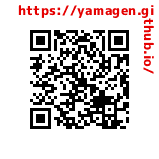
\includegraphics[height=20cm]{images/qr20250715111608434.png}
};

% QRコード(左下)
\node[
  anchor=south east
] at ([xshift=-45cm,yshift=1cm]current page.south east) {
  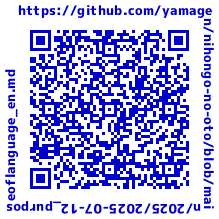
\includegraphics[height=17cm]{images/qr20250715120047363.png}
};

\end{tikzpicture}

\end{document}



